\documentclass{beamer}

\usepackage{amsmath, amssymb}
\usepackage{graphicx}
\usepackage{url}
\usepackage{xspace}
\usepackage{pifont}
\usepackage{minted}
\usepackage{verbatim}
\usepackage{wasysym}

\usetheme{AnnArbor}
\usefonttheme[onlymath]{serif}

\title[Intro DNNs]{\textbf{Practical Deep Neural Networks} \\
\textbf{\normalsize GPU computing perspective}\\
\normalsize Python Platform for Scientific Computing}
\author{Yuhuang Hu \and Chu Kiong Loo}
\institute[UM]{Advanced Robotic Lab\\
Department of Artificial Intelligence\\
Faculty of Computer Science \& IT\\
University of Malaya}

\newcommand{\ubuntu}{\texttt{Ubuntu}\xspace}
\newcommand{\ubuntults}{\texttt{Ubuntu 14.04.2 LTS}\xspace}

\date{}

\begin{document}

\frame{\titlepage}

\begin{frame}
\frametitle{Outline}

\tableofcontents

\end{frame}

\section{Ubuntu}

\begin{frame}
\frametitle{Why \ubuntu?}

\begin{minipage}{0.6\textwidth}
\begin{itemize}
\item[\ding{55}] There are more than thousands kinds of \texttt{*nix} distribution, and \ubuntu is only one of them.
\item[\ding{55}] \ubuntu contains non-free software.
\item[\checkmark] \ubuntu is widely used by academic community in computing.
\item[\checkmark] Most of Deep Learning libraries explicitly support \ubuntu.
\item[\checkmark] Stable, fast, less issues.
\end{itemize}
\end{minipage}
\begin{minipage}{0.3\textwidth}
  \centering
  \begin{figure}
    
\includegraphics[width=\textwidth]{ubuntulogo.png}
  \end{figure}
\end{minipage}

\end{frame}

\begin{frame}
\frametitle{Setting up \ubuntu: Tips}

\begin{itemize}
\item[\ding{80}] Stick to stable release \texttt{xx.04.x LTS}, \emph{e.g.} we are using \ubuntults.
\item[\ding{80}] Update right after your fresh installation.
\item[\ding{80}] \textbf{DO NOT} install graphical driver through \ubuntu's package repository.
\item[\ding{80}] \textbf{DO NOT} update anything anymore in the future if you don't have to. 
\end{itemize}

\end{frame}

\begin{frame}[fragile]

\frametitle{Setting up \ubuntu: necessary software before start}

\begin{block}{Setup basic development environment}
\begin{verbatim}
$ sudo apt-get update
$ sudo apt-get upgrade
$ sudo apt-get build-essential binutils
$ sudo apt-get install git cmake
$ sudo apt-get install openjdk-7-jdk
\end{verbatim}
\end{block}

\end{frame}

\section{Build Computing Platform}

\begin{frame}[fragile]
\frametitle{Anaconda}

We use a specific distribution of \texttt{Python} --- \texttt{Anaconda}, which is designed for large-scale data processing, predictive analytics, and scientific computing. You can download from here:
\begin{verbatim}
http://continuum.io/downloads
\end{verbatim}
Since most of software are not compatible with \texttt{Python 3.*}, please download \texttt{Python 2.7}. And Install with
\begin{block}{Setup Anaconda}
\begin{verbatim}
$ bash Anaconda-2.2.0-Linux-x86.sh
\end{verbatim}
\end{block}

\end{frame}

\begin{frame}[fragile]
\frametitle{Anaconda}

\begin{minipage}{0.6\textwidth}
\begin{itemize}
\item[\checkmark] Easy install, easy remove ({\small \emph{delete \texttt{Anaconda} folder from home folder}})
\item[\checkmark] Awesome package management, no mess in system library.
\item[\checkmark] Simplified complex package installation. 
\item[\checkmark] Complete computing libraries pre-installed, immediately ready-to-go.
\end{itemize}
\end{minipage}
\begin{minipage}{0.35\textwidth}
\begin{figure}
  
\includegraphics[width=\textwidth]{anaconda_logo.png}
\end{figure}
\end{minipage}

\end{frame}

\begin{frame}[fragile]
\frametitle{Theano}

\begin{itemize}
\item[\checkmark] Theano has been pre-installed in \texttt{Anaconda}.
\item[\ding{112}] Setup Theano configuration.
\item[\ding{112}] Setup GPU environment for Theano. [Next Section].
\end{itemize}

\end{frame}

\begin{frame}[fragile]
  \frametitle{Configure Theano}
  Before you start, you need to create a new file \texttt{.theanorc} under your home folder:
\begin{verbatim}
$ touch .theanorc
\end{verbatim}
  
  Assume you have only CPU available, you can edit this file as follows:
  \begin{block}{.theanorc}
\begin{verbatim}
[global]
floatX = float32
device = cpu
\end{verbatim}
  \end{block}
  
  \textbf{You are ready to go!} \smiley
\end{frame}

\section{Eclipse + PyDev}

\begin{frame}
\frametitle{FYI}
\begin{center}
\emph{This configuration is only a suggest, choose whatever you feel comfortable.}
\end{center}
\end{frame}

\begin{frame}
\frametitle{Why Eclipse? And why PyDev?}

\begin{minipage}{0.3\textwidth}
\begin{figure}

\includegraphics[width=0.8\textwidth]{eclipse_logo.png}\\

\includegraphics[width=0.8\textwidth]{pydev_logo.png}
\end{figure}
\end{minipage}
\begin{minipage}{0.6\textwidth}
\begin{itemize}
\item[\ding{79}] And IDE that can do a lot.
\item[\ding{79}] Excellent hightlighter, language support, source code control, auto-completion.
\item[\ding{79}] Easy to configure, easy to extend.
\end{itemize}
\end{minipage}

\end{frame}

\begin{frame}[fragile]
\frametitle{Install Eclipse}

If you installed JDK 7 like previous, then you can download Eclipse Kepler:
\begin{verbatim}
http://eclipse.org/kepler/
\end{verbatim}
If you installed JDK 8, you can use Eclipse Luna
\begin{verbatim}
http://eclipse.org/luna/
\end{verbatim}

Download \emph{Eclipse Standard 4.3.2} for Eclipse Kepler or \emph{Eclipse IDE for Eclipse Committers 4.4.2} for Eclips Luna.

Unzip the entire \texttt{eclipse} folder to you home folder, the installation is then ready. 

\end{frame}

\begin{frame}[fragile]
\frametitle{Setup PyDev}

Eclipse is designed as a Java IDE, however, you can install new software for other languages like Python.

\begin{itemize}
\item[\ding{43}] Select help$\rightarrow$Install New Software, type
\begin{verbatim}
http://pydev.org/updates
\end{verbatim}
in \emph{Work with:}, hit Enter, PyDev is retrieved.
\item[\ding{43}] Select PyDev and leave PyDev Mylyn Integration as blank.
\item[\ding{43}] Click Next and then follow the instruction. If there is an warning for unauthorized software, make sure you select all of them, they are not malware, just some routines for PyDev.
\item[\ding{43}] Restart Eclipse, you should be able to create PyDev Project.
\end{itemize}

\end{frame}

\begin{frame}[fragile]
\frametitle{Hook up Anaconda}

Assumed you installed PyDev successfully.
\begin{itemize}
  \item[\ding{43}] Select Window$\rightarrow$Preferences$\rightarrow$PyDev$\rightarrow$Interpreters$\rightarrow$Python Interpreter
  \item[\ding{43}] Click New, type ``Anaconda'' in Interpreter Name and ``\texttt{/path/to/anaconda/bin/python}'' in Interpreter Executable (or use Browse to select your Anaconda's python executable). Click OK, then Eclipse will associate all installed packages in Anaconda.
  \item[\ding{43}] Click Apply and then Click OK to exit. You now can use Anaconda in Eclipse.
\end{itemize}

\end{frame}

\begin{frame}[fragile]
\frametitle{Create your first PyDev Project}

Assume you installed PyDev and configured Anaconda
\begin{itemize}
\item[\ding{43}] Select File$\rightarrow$PyDev Project$\rightarrow$Next
\item[\ding{43}] Type in project name and select Interpreter as ``Anaconda''.
\item[\ding{43}] Click Finish, you project is created.
\item[\ding{43}] You can now create your script or develop your package.
\end{itemize}

\end{frame}

\section{NVIDIA GPU Driver and CUDA Toolkit}

\begin{frame}
\frametitle{Heads Up}

\begin{center}
\textbf{DO NOT} use \ubuntu's package repository to install NVIDIA GPU Driver and CUDA Toolkit, it's not state-of-the-art, and stable.

Procedures discussed here are experimental, no success guarantee.
\end{center}
\end{frame}

\begin{frame}
\frametitle{Why NVIDIA?}

\begin{minipage}{0.6\textwidth}
\begin{itemize}
\item[\checkmark] Widely used in industry and academic world.
\item[\checkmark] \textbf{All} popular Deep Learning libraries support CUDA, which is designed for NVIDIA graphics card only.
\item[\checkmark] Excellent performance and easy-to-use library interface.
\item[\checkmark] Industry standard.
\end{itemize}
\end{minipage}
\begin{minipage}{0.3\textwidth}
\begin{figure}
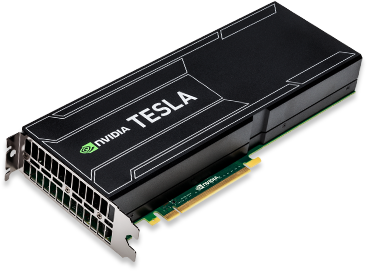
\includegraphics[width=\textwidth]{nvidia_tesla.png}
\end{figure}
\end{minipage}

\end{frame}

\begin{frame}
\frametitle{Prerequisites}

\begin{itemize}
\item[\ding{112}] A computer with a NVIDIA graphics card that supports CUDA technology.
\item[\ding{112}] Enough disk space and at least 4 GB RAM. (Assume 64bit machine)
\item[\ding{112}] Compute Capability of your card has to be at least 3.0 if you are intending to use \texttt{cuDNN} routines.
\item[\ding{112}] A heart that is strong enough to take failure.
\end{itemize}

\end{frame}

\begin{frame}[fragile]
\frametitle{Install GPU driver}

\begin{itemize}
\item[\ding{43}] Check out your GPU's info:
\begin{verbatim}
$ lspci | grep "VGA"
\end{verbatim}
You should get similar messages like:
\begin{verbatim}
00:02.0 VGA compatible controller: Cirrus 
Logic GD 5446
00:03.0 VGA compatible controller: NVIDIA 
Corporation GK104GL [GRID K520] (rev a1)
\end{verbatim}

\item[\ding{43}] Go to NVIDIA website to download corresponding driver:

\url{http://www.nvidia.com/Download/index.aspx?lang=en-us}
\end{itemize}

\end{frame}

\begin{frame}[fragile]
\frametitle{Install GPU driver}

\begin{itemize}
\item[\ding{43}] Close \texttt{nouveau} [further experiment]
\item[\ding{43}] Install GPU driver
\begin{verbatim}
$ bash NVIDIA-Linux-xx.run
\end{verbatim}
Reboot after you installed the the driver, your GPU is now taking in charge

\item[\ding{43}] You can check your installed driver by:
\begin{verbatim}
$ nvidia-smi
\end{verbatim}
You should see a table that states the status of your GPU and driver version.
\end{itemize}

\textbf{DO NOT} update your system anymore since this moment, new kernel update may not be compatiable with your driver and then you will lost your GUI for sure. If this happens, you have to force boot older kernel version.
\end{frame}

\begin{frame}[fragile]
\frametitle{Install CUDA Toolkit}

At this moment, CUDA Toolkit 7 is released, this guide is based on CUDA Toolkit 7.

\begin{itemize}
\item[\ding{43}] Download CUDA 7 from NVIDIA's developer website:

\url{https://developer.nvidia.com/cuda-downloads}

\item[\ding{43}] Install CUDA by:
\begin{verbatim}
$ sudo bash cuda_xx_linux64.run
\end{verbatim}
DO NOT INSTALL GPU DRIVER INSIDE THE CUDA TOOLKIT. Remember to create symbolic link if the installer asked.

\end{itemize}

\end{frame}

\begin{frame}[fragile]
\frametitle{Install CUDA Toolkit}

Add following contents in your bash configuration file \texttt{~/.bashrc}.
\small
\begin{block}{.bashrc}
\begin{verbatim}
# This configuration uses CUDA's symbolic link
export PATH=$PATH:/usr/local/cuda/bin
export LD_LIBRARY_PATH=$LD_LIBRARY_PATH:/usr/local/cuda/lib64
export CUDA_ROOT=/usr/local/cuda
\end{verbatim}
\end{block}

\end{frame}

\begin{frame}[fragile]
\frametitle{Install CUDA Toolkit}
And configure your \texttt{.theanorc} as
\begin{block}{.theanorc}
\begin{verbatim}
[global]
floatX = float32
device = gpu0

[nvcc]
fastmath = True

[cuda]
root = /usr/local/cuda
\end{verbatim}
\end{block}
in order to enable GPU usage in your python scripts.
\end{frame}

\begin{frame}[fragile]
  \frametitle{Before the end: cuDNN}

  The NVIDIA CUDA Deep Neural Network library (cuDNN) is a GPU-accelerated library of primitives for deep neural networks. Popular libraries, such as Theano, Caffe and Torch 7 have added the support of cuDNN, the performance is improved significantly during implementing Convolutional Neural Networks (ConvNets).

  \begin{itemize}
    \item Request a copy of your cuDNN from NVIDIA:

      \url{https://developer.nvidia.com/cuDNN}
    \item Extract cuDNN:
\begin{verbatim}
$ tar zxvf cudnn-xx.tgz
\end{verbatim}
    \item Copy extracted files to CUDA folder:
\begin{verbatim}
$ sudo cp cudnn.h /usr/local/cuda-x/include
$ sudo cp libcudnn* /usr/local/cuda-x/lib64
\end{verbatim}
      Now your cuDNN is installed correctly.
  \end{itemize}
\end{frame}

\begin{frame}
\frametitle{Before the end: how to select GPU for research}

Select the right GPU can save you lots of money and boost your performance, you should read through this article before your purchase:

\url{https://timdettmers.wordpress.com/2014/08/14/which-gpu-for-deep-learning/}

From conclusion of the article:
\small
\begin{itemize}
\item[\ding{96}] best GPU overall: GTX Titan X
\item[\ding{96}] cost efficient but still expensive: GTX Titan X or GTX 980
\item[\ding{96}] cheapest card with no troubles: GTX 960 4GB or GTX 680
\item[\ding{96}] I work with data sets $>$ 250GB: GTX Titan
\item[\ding{96}] I have no money: GTX 680 3GB
\item[\ding{96}] I do Kaggle: GTX 980 or GTX 960 4GB
\item[\ding{96}] I am a researcher: 1-4x GTX 980
\item[\ding{96}] I am a researcher with data sets $>$ 250GB: 1-4x GTX Titan
\end{itemize}

\end{frame}

\begin{frame}
\frametitle{Before the end: Amazon Web Services EC2 GPU Instance}

\begin{minipage}{0.3\textwidth}
  \begin{figure}
    
\includegraphics[width=\textwidth]{aws_logo.png}
  \end{figure}
\end{minipage}
\begin{minipage}{0.6\textwidth}
\begin{itemize}
\item[\ding{71}] Two kinds of GPU instances are available
  \begin{itemize}
    \item[\ding{246}] g2.2xlarge: GPU: 1, CPU: 8 cores, RAM: 15 GB, SSD Storage
    \item[\ding{246}] g2.8xlarge: GPU: 4, CPU: 32 cores, RAM: 60 GB, SSD Storage
  \end{itemize}
\item[\ding{71}] We configured public images for deep learning usage:
  \begin{itemize}
    \item[\ding{246}] DGYDLGPUv3 (ami-c5c2ee97) for g2.2xlarge
    \item[\ding{246}] Image for g2.8xlarge is on the way
  \end{itemize}
\item[\ding{71}] Use Spot Request Instance to enjoy both speed and low cost.
\end{itemize}
\end{minipage}

\end{frame}

\section{Q \& A}
\begin{frame}
\begin{figure}

\includegraphics[width=0.5\textwidth]{qanda.pdf}
\end{figure}
\end{frame}

\end{document}
%%% Local Variables:
%%% mode: latex
%%% TeX-master: t
%%% End:
